\documentclass[twoside]{book}

% Packages required by doxygen
\usepackage{calc}
\usepackage{doxygen}
\usepackage{graphicx}
\usepackage[utf8]{inputenc}
\usepackage{makeidx}
\usepackage{multicol}
\usepackage{multirow}
\usepackage{textcomp}
\usepackage[table]{xcolor}

% Font selection
\usepackage[T1]{fontenc}
\usepackage{mathptmx}
\usepackage[scaled=.90]{helvet}
\usepackage{courier}
\usepackage{amssymb}
\usepackage{sectsty}
\renewcommand{\familydefault}{\sfdefault}
\allsectionsfont{%
  \fontseries{bc}\selectfont%
  \color{darkgray}%
}
\renewcommand{\DoxyLabelFont}{%
  \fontseries{bc}\selectfont%
  \color{darkgray}%
}

% Page & text layout
\usepackage{geometry}
\geometry{%
  a4paper,%
  top=2.5cm,%
  bottom=2.5cm,%
  left=2.5cm,%
  right=2.5cm%
}
\tolerance=750
\hfuzz=15pt
\hbadness=750
\setlength{\emergencystretch}{15pt}
\setlength{\parindent}{0cm}
\setlength{\parskip}{0.2cm}
\makeatletter
\renewcommand{\paragraph}{%
  \@startsection{paragraph}{4}{0ex}{-1.0ex}{1.0ex}{%
    \normalfont\normalsize\bfseries\SS@parafont%
  }%
}
\renewcommand{\subparagraph}{%
  \@startsection{subparagraph}{5}{0ex}{-1.0ex}{1.0ex}{%
    \normalfont\normalsize\bfseries\SS@subparafont%
  }%
}
\makeatother

% Headers & footers
\usepackage{fancyhdr}
\pagestyle{fancyplain}
\fancyhead[LE]{\fancyplain{}{\bfseries\thepage}}
\fancyhead[CE]{\fancyplain{}{}}
\fancyhead[RE]{\fancyplain{}{\bfseries\leftmark}}
\fancyhead[LO]{\fancyplain{}{\bfseries\rightmark}}
\fancyhead[CO]{\fancyplain{}{}}
\fancyhead[RO]{\fancyplain{}{\bfseries\thepage}}
\fancyfoot[LE]{\fancyplain{}{}}
\fancyfoot[CE]{\fancyplain{}{}}
\fancyfoot[RE]{\fancyplain{}{\bfseries\scriptsize Generated on Fri Oct 4 2013 01\-:58\-:15 for Lab 13\-: Performance Evaluation by Doxygen }}
\fancyfoot[LO]{\fancyplain{}{\bfseries\scriptsize Generated on Fri Oct 4 2013 01\-:58\-:15 for Lab 13\-: Performance Evaluation by Doxygen }}
\fancyfoot[CO]{\fancyplain{}{}}
\fancyfoot[RO]{\fancyplain{}{}}
\renewcommand{\footrulewidth}{0.4pt}
\renewcommand{\chaptermark}[1]{%
  \markboth{#1}{}%
}
\renewcommand{\sectionmark}[1]{%
  \markright{\thesection\ #1}%
}

% Indices & bibliography
\usepackage{natbib}
\usepackage[titles]{tocloft}
\setcounter{tocdepth}{3}
\setcounter{secnumdepth}{5}
\makeindex

% Hyperlinks (required, but should be loaded last)
\usepackage{ifpdf}
\ifpdf
  \usepackage[pdftex,pagebackref=true]{hyperref}
\else
  \usepackage[ps2pdf,pagebackref=true]{hyperref}
\fi
\hypersetup{%
  colorlinks=true,%
  linkcolor=blue,%
  citecolor=blue,%
  unicode%
}

% Custom commands
\newcommand{\clearemptydoublepage}{%
  \newpage{\pagestyle{empty}\cleardoublepage}%
}


%===== C O N T E N T S =====

\begin{document}

% Titlepage & ToC
\hypersetup{pageanchor=false}
\pagenumbering{roman}
\begin{titlepage}
\vspace*{7cm}
\begin{center}%
{\Large Lab 13\-: Performance Evaluation }\\
\vspace*{1cm}
{\large Generated by Doxygen 1.8.5}\\
\vspace*{0.5cm}
{\small Fri Oct 4 2013 01:58:15}\\
\end{center}
\end{titlepage}
\clearemptydoublepage
\tableofcontents
\clearemptydoublepage
\pagenumbering{arabic}
\hypersetup{pageanchor=true}

%--- Begin generated contents ---
\chapter{Hierarchical Index}
\section{Class Hierarchy}
This inheritance list is sorted roughly, but not completely, alphabetically\-:\begin{DoxyCompactList}
\item \contentsline{section}{Greater$<$ Key\-Type $>$}{\pageref{class_greater}}{}
\item \contentsline{section}{Heap$<$ Data\-Type, Key\-Type, Comparator $>$}{\pageref{class_heap}}{}
\item \contentsline{section}{Heap$<$ Data\-Type $>$}{\pageref{class_heap}}{}
\begin{DoxyCompactList}
\item \contentsline{section}{Priority\-Queue$<$ Data\-Type, Key\-Type, Comparator $>$}{\pageref{class_priority_queue}}{}
\end{DoxyCompactList}
\item \contentsline{section}{Less$<$ Key\-Type $>$}{\pageref{class_less}}{}
\item \contentsline{section}{Less$<$ int $>$}{\pageref{class_less}}{}
\item \contentsline{section}{Task\-Data}{\pageref{struct_task_data}}{}
\item \contentsline{section}{Test\-Data}{\pageref{class_test_data}}{}
\item \contentsline{section}{Test\-Data\-Item$<$ Key\-Type $>$}{\pageref{class_test_data_item}}{}
\end{DoxyCompactList}

\chapter{Class Index}
\section{Class List}
Here are the classes, structs, unions and interfaces with brief descriptions\-:\begin{DoxyCompactList}
\item\contentsline{section}{\hyperlink{classbinary_search}{binary\-Search} }{\pageref{classbinary_search}}{}
\item\contentsline{section}{\hyperlink{classlinear_search}{linear\-Search} }{\pageref{classlinear_search}}{}
\item\contentsline{section}{\hyperlink{class_search}{Search} }{\pageref{class_search}}{}
\item\contentsline{section}{\hyperlink{class_s_t_l_search}{S\-T\-L\-Search} }{\pageref{class_s_t_l_search}}{}
\item\contentsline{section}{\hyperlink{class_test_vector}{Test\-Vector} }{\pageref{class_test_vector}}{}
\item\contentsline{section}{\hyperlink{class_timer}{Timer} }{\pageref{class_timer}}{}
\end{DoxyCompactList}

\chapter{File Index}
\section{File List}
Here is a list of all files with brief descriptions\-:\begin{DoxyCompactList}
\item\contentsline{section}{\hyperlink{config_8h}{config.\-h} }{\pageref{config_8h}}{}
\item\contentsline{section}{\hyperlink{constructor_8cpp}{constructor.\-cpp} }{\pageref{constructor_8cpp}}{}
\item\contentsline{section}{\hyperlink{inc_8cpp}{inc.\-cpp} }{\pageref{inc_8cpp}}{}
\item\contentsline{section}{\hyperlink{search_8cpp}{search.\-cpp} }{\pageref{search_8cpp}}{}
\item\contentsline{section}{\hyperlink{sort_8cpp}{sort.\-cpp} }{\pageref{sort_8cpp}}{}
\item\contentsline{section}{\hyperlink{test_8cpp}{test.\-cpp} }{\pageref{test_8cpp}}{}
\item\contentsline{section}{\hyperlink{test13_8cpp}{test13.\-cpp} }{\pageref{test13_8cpp}}{}
\item\contentsline{section}{\hyperlink{testtimer_8c_09_09}{testtimer.\-c++} }{\pageref{testtimer_8c_09_09}}{}
\item\contentsline{section}{\hyperlink{testtimer_8cc}{testtimer.\-cc} }{\pageref{testtimer_8cc}}{}
\item\contentsline{section}{\hyperlink{testtimer_8cpp}{testtimer.\-cpp} }{\pageref{testtimer_8cpp}}{}
\item\contentsline{section}{\hyperlink{testvector_8cpp}{testvector.\-cpp} }{\pageref{testvector_8cpp}}{}
\item\contentsline{section}{\hyperlink{testvector_8h}{testvector.\-h} }{\pageref{testvector_8h}}{}
\item\contentsline{section}{\hyperlink{text_8cc}{text.\-cc} }{\pageref{text_8cc}}{}
\item\contentsline{section}{\hyperlink{_timer_8cpp}{Timer.\-cpp} }{\pageref{_timer_8cpp}}{}
\item\contentsline{section}{\hyperlink{_timer_8cs}{Timer.\-cs} }{\pageref{_timer_8cs}}{}
\item\contentsline{section}{\hyperlink{_timer_8h}{Timer.\-h} }{\pageref{_timer_8h}}{}
\end{DoxyCompactList}

\chapter{Class Documentation}
\hypertarget{classbinary_search}{\section{binary\-Search Class Reference}
\label{classbinary_search}\index{binary\-Search@{binary\-Search}}
}
Inheritance diagram for binary\-Search\-:\begin{figure}[H]
\begin{center}
\leavevmode
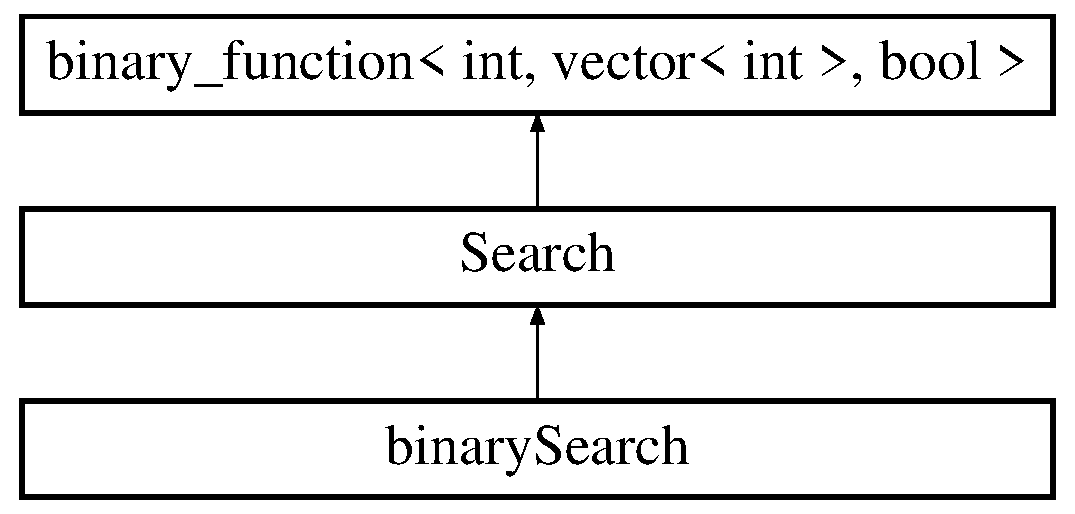
\includegraphics[height=3.000000cm]{classbinary_search}
\end{center}
\end{figure}
\subsection*{Public Member Functions}
\begin{DoxyCompactItemize}
\item 
bool \hyperlink{classbinary_search_a8e145edfb29183d7e1b265bd4cf4293f}{operator()} (int search\-Value, const vector$<$ int $>$ \&keys) const 
\end{DoxyCompactItemize}


\subsection{Member Function Documentation}
\hypertarget{classbinary_search_a8e145edfb29183d7e1b265bd4cf4293f}{\index{binary\-Search@{binary\-Search}!operator()@{operator()}}
\index{operator()@{operator()}!binarySearch@{binary\-Search}}
\subsubsection[{operator()}]{\setlength{\rightskip}{0pt plus 5cm}bool binary\-Search\-::operator() (
\begin{DoxyParamCaption}
\item[{int}]{search\-Value, }
\item[{const vector$<$ int $>$ \&}]{keys}
\end{DoxyParamCaption}
) const\hspace{0.3cm}{\ttfamily [inline]}, {\ttfamily [virtual]}}}\label{classbinary_search_a8e145edfb29183d7e1b265bd4cf4293f}


Implements \hyperlink{class_search}{Search}.



The documentation for this class was generated from the following file\-:\begin{DoxyCompactItemize}
\item 
\hyperlink{search_8cpp}{search.\-cpp}\end{DoxyCompactItemize}

\hypertarget{classlinear_search}{\section{linear\-Search Class Reference}
\label{classlinear_search}\index{linear\-Search@{linear\-Search}}
}
Inheritance diagram for linear\-Search\-:\begin{figure}[H]
\begin{center}
\leavevmode
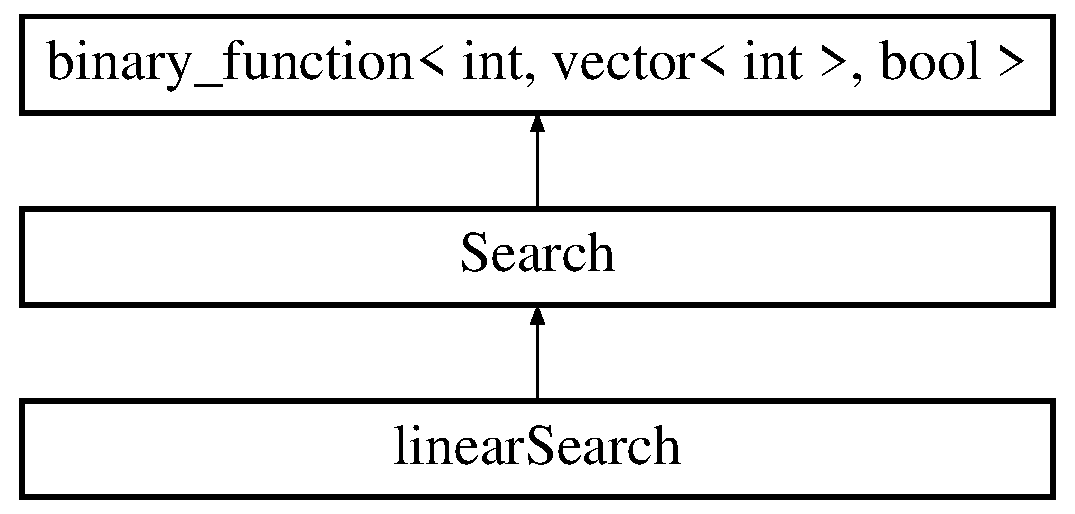
\includegraphics[height=3.000000cm]{classlinear_search}
\end{center}
\end{figure}
\subsection*{Public Member Functions}
\begin{DoxyCompactItemize}
\item 
bool \hyperlink{classlinear_search_a447bc4f724457f1786dc36c10626bfa8}{operator()} (int search\-Value, const vector$<$ int $>$ \&keys) const 
\end{DoxyCompactItemize}


\subsection{Member Function Documentation}
\hypertarget{classlinear_search_a447bc4f724457f1786dc36c10626bfa8}{\index{linear\-Search@{linear\-Search}!operator()@{operator()}}
\index{operator()@{operator()}!linearSearch@{linear\-Search}}
\subsubsection[{operator()}]{\setlength{\rightskip}{0pt plus 5cm}bool linear\-Search\-::operator() (
\begin{DoxyParamCaption}
\item[{int}]{search\-Value, }
\item[{const vector$<$ int $>$ \&}]{keys}
\end{DoxyParamCaption}
) const\hspace{0.3cm}{\ttfamily [inline]}, {\ttfamily [virtual]}}}\label{classlinear_search_a447bc4f724457f1786dc36c10626bfa8}


Implements \hyperlink{class_search}{Search}.



The documentation for this class was generated from the following file\-:\begin{DoxyCompactItemize}
\item 
\hyperlink{search_8cpp}{search.\-cpp}\end{DoxyCompactItemize}

\hypertarget{class_search}{\section{Search Class Reference}
\label{class_search}\index{Search@{Search}}
}
Inheritance diagram for Search\-:\begin{figure}[H]
\begin{center}
\leavevmode
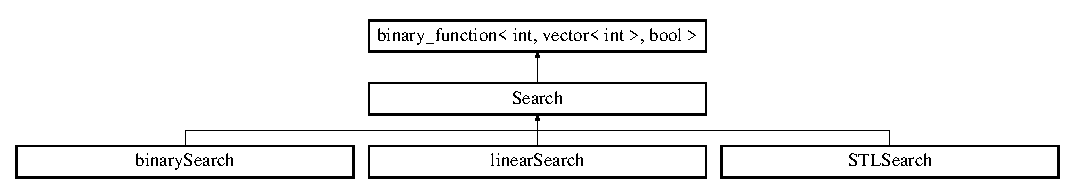
\includegraphics[height=2.153846cm]{class_search}
\end{center}
\end{figure}


The documentation for this class was generated from the following file\-:\begin{DoxyCompactItemize}
\item 
\hyperlink{search_8cpp}{search.\-cpp}\end{DoxyCompactItemize}

\hypertarget{class_s_t_l_search}{\section{S\-T\-L\-Search Class Reference}
\label{class_s_t_l_search}\index{S\-T\-L\-Search@{S\-T\-L\-Search}}
}
Inheritance diagram for S\-T\-L\-Search\-:\begin{figure}[H]
\begin{center}
\leavevmode
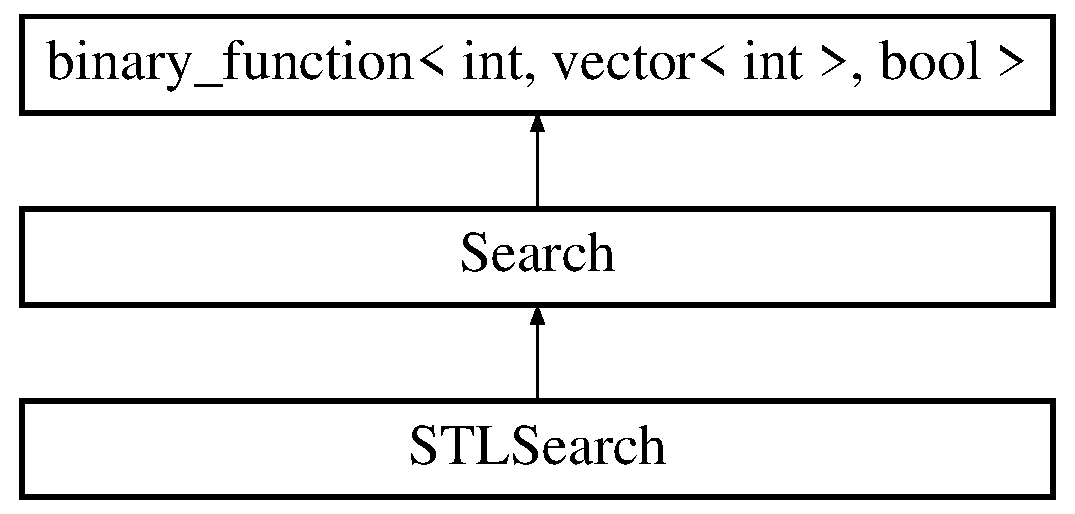
\includegraphics[height=3.000000cm]{class_s_t_l_search}
\end{center}
\end{figure}
\subsection*{Public Member Functions}
\begin{DoxyCompactItemize}
\item 
bool \hyperlink{class_s_t_l_search_a0f3684e33bd5e47317ab5a94d6f52dba}{operator()} (int search\-Value, const vector$<$ int $>$ \&keys) const 
\end{DoxyCompactItemize}


\subsection{Member Function Documentation}
\hypertarget{class_s_t_l_search_a0f3684e33bd5e47317ab5a94d6f52dba}{\index{S\-T\-L\-Search@{S\-T\-L\-Search}!operator()@{operator()}}
\index{operator()@{operator()}!STLSearch@{S\-T\-L\-Search}}
\subsubsection[{operator()}]{\setlength{\rightskip}{0pt plus 5cm}bool S\-T\-L\-Search\-::operator() (
\begin{DoxyParamCaption}
\item[{int}]{search\-Value, }
\item[{const vector$<$ int $>$ \&}]{keys}
\end{DoxyParamCaption}
) const\hspace{0.3cm}{\ttfamily [inline]}, {\ttfamily [virtual]}}}\label{class_s_t_l_search_a0f3684e33bd5e47317ab5a94d6f52dba}


Implements \hyperlink{class_search}{Search}.



The documentation for this class was generated from the following file\-:\begin{DoxyCompactItemize}
\item 
\hyperlink{search_8cpp}{search.\-cpp}\end{DoxyCompactItemize}

\hypertarget{class_test_vector}{\section{Test\-Vector Class Reference}
\label{class_test_vector}\index{Test\-Vector@{Test\-Vector}}
}


{\ttfamily \#include $<$testvector.\-h$>$}

\subsection*{Public Member Functions}
\begin{DoxyCompactItemize}
\item 
\hyperlink{class_test_vector_abf540180761043bb7ac2665e147bdd33}{Test\-Vector} (int size)
\item 
\hyperlink{class_test_vector_a4a48046f67cc822ce9a6907f022a5d61}{Test\-Vector} (const \hyperlink{class_test_vector}{Test\-Vector} \&rhs)
\item 
\hyperlink{class_test_vector}{Test\-Vector} \& \hyperlink{class_test_vector_a8d4a95de7e0e9985ffcd86280efb631d}{operator++} ()
\item 
\hyperlink{class_test_vector}{Test\-Vector} \hyperlink{class_test_vector_a1b9640623055cd4618606cd2f0ed08b3}{operator++} (int ignored)
\item 
int \hyperlink{class_test_vector_ae244371b88cb0ab127a877e5206b7ed8}{operator\mbox{[}$\,$\mbox{]}} (int loc) const 
\end{DoxyCompactItemize}


\subsection{Constructor \& Destructor Documentation}
\hypertarget{class_test_vector_abf540180761043bb7ac2665e147bdd33}{\index{Test\-Vector@{Test\-Vector}!Test\-Vector@{Test\-Vector}}
\index{Test\-Vector@{Test\-Vector}!TestVector@{Test\-Vector}}
\subsubsection[{Test\-Vector}]{\setlength{\rightskip}{0pt plus 5cm}Test\-Vector\-::\-Test\-Vector (
\begin{DoxyParamCaption}
\item[{int}]{size}
\end{DoxyParamCaption}
)}}\label{class_test_vector_abf540180761043bb7ac2665e147bdd33}
\hypertarget{class_test_vector_a4a48046f67cc822ce9a6907f022a5d61}{\index{Test\-Vector@{Test\-Vector}!Test\-Vector@{Test\-Vector}}
\index{Test\-Vector@{Test\-Vector}!TestVector@{Test\-Vector}}
\subsubsection[{Test\-Vector}]{\setlength{\rightskip}{0pt plus 5cm}Test\-Vector\-::\-Test\-Vector (
\begin{DoxyParamCaption}
\item[{const {\bf Test\-Vector} \&}]{rhs}
\end{DoxyParamCaption}
)}}\label{class_test_vector_a4a48046f67cc822ce9a6907f022a5d61}


\subsection{Member Function Documentation}
\hypertarget{class_test_vector_a8d4a95de7e0e9985ffcd86280efb631d}{\index{Test\-Vector@{Test\-Vector}!operator++@{operator++}}
\index{operator++@{operator++}!TestVector@{Test\-Vector}}
\subsubsection[{operator++}]{\setlength{\rightskip}{0pt plus 5cm}{\bf Test\-Vector} \& Test\-Vector\-::operator++ (
\begin{DoxyParamCaption}
{}
\end{DoxyParamCaption}
)}}\label{class_test_vector_a8d4a95de7e0e9985ffcd86280efb631d}
\hypertarget{class_test_vector_a1b9640623055cd4618606cd2f0ed08b3}{\index{Test\-Vector@{Test\-Vector}!operator++@{operator++}}
\index{operator++@{operator++}!TestVector@{Test\-Vector}}
\subsubsection[{operator++}]{\setlength{\rightskip}{0pt plus 5cm}{\bf Test\-Vector} Test\-Vector\-::operator++ (
\begin{DoxyParamCaption}
\item[{int}]{ignored}
\end{DoxyParamCaption}
)}}\label{class_test_vector_a1b9640623055cd4618606cd2f0ed08b3}
\hypertarget{class_test_vector_ae244371b88cb0ab127a877e5206b7ed8}{\index{Test\-Vector@{Test\-Vector}!operator\mbox{[}$\,$\mbox{]}@{operator[]}}
\index{operator\mbox{[}$\,$\mbox{]}@{operator[]}!TestVector@{Test\-Vector}}
\subsubsection[{operator[]}]{\setlength{\rightskip}{0pt plus 5cm}int Test\-Vector\-::operator\mbox{[}$\,$\mbox{]} (
\begin{DoxyParamCaption}
\item[{int}]{loc}
\end{DoxyParamCaption}
) const}}\label{class_test_vector_ae244371b88cb0ab127a877e5206b7ed8}


The documentation for this class was generated from the following files\-:\begin{DoxyCompactItemize}
\item 
\hyperlink{testvector_8h}{testvector.\-h}\item 
\hyperlink{testvector_8cpp}{testvector.\-cpp}\end{DoxyCompactItemize}

\hypertarget{class_timer}{\section{Timer Class Reference}
\label{class_timer}\index{Timer@{Timer}}
}


{\ttfamily \#include $<$Timer.\-h$>$}

\subsection*{Public Member Functions}
\begin{DoxyCompactItemize}
\item 
\hyperlink{class_timer_a5f16e8da27d2a5a5242dead46de05d97}{Timer} ()
\item 
void \hyperlink{class_timer_a3a8b5272198d029779dc9302a54305a8}{start} ()  throw (runtime\-\_\-error)
\item 
void \hyperlink{class_timer_a63f0eb44b27402196590a03781515dba}{stop} ()  throw (logic\-\_\-error)
\item 
double \hyperlink{class_timer_ad306e18f8d8a0296e001683f92d7f86e}{get\-Elapsed\-Time} () const   throw (logic\-\_\-error)
\end{DoxyCompactItemize}


\subsection{Constructor \& Destructor Documentation}
\hypertarget{class_timer_a5f16e8da27d2a5a5242dead46de05d97}{\index{Timer@{Timer}!Timer@{Timer}}
\index{Timer@{Timer}!Timer@{Timer}}
\subsubsection[{Timer}]{\setlength{\rightskip}{0pt plus 5cm}Timer\-::\-Timer (
\begin{DoxyParamCaption}
{}
\end{DoxyParamCaption}
)}}\label{class_timer_a5f16e8da27d2a5a5242dead46de05d97}
\begin{DoxyPrecond}{Precondition}
Unitialized \hyperlink{class_timer}{Timer} Class 
\end{DoxyPrecond}
\begin{DoxyPostcond}{Postcondition}
Duration assigned to -\/1 timer\-Was\-Started assigned false
\end{DoxyPostcond}
Algorithm\-:
\begin{DoxyItemize}
\item Assign data members values
\end{DoxyItemize}

Exceptional/\-Error Conditions\-:
\begin{DoxyItemize}
\item none 
\end{DoxyItemize}

\subsection{Member Function Documentation}
\hypertarget{class_timer_ad306e18f8d8a0296e001683f92d7f86e}{\index{Timer@{Timer}!get\-Elapsed\-Time@{get\-Elapsed\-Time}}
\index{get\-Elapsed\-Time@{get\-Elapsed\-Time}!Timer@{Timer}}
\subsubsection[{get\-Elapsed\-Time}]{\setlength{\rightskip}{0pt plus 5cm}double Timer\-::get\-Elapsed\-Time (
\begin{DoxyParamCaption}
{}
\end{DoxyParamCaption}
) const throw  logic\-\_\-error) }}\label{class_timer_ad306e18f8d8a0296e001683f92d7f86e}
Parameters\-: none

\begin{DoxyReturn}{Returns}
The time in seconds as a double
\end{DoxyReturn}
\begin{DoxyPrecond}{Precondition}
none
\end{DoxyPrecond}
\begin{DoxyPostcond}{Postcondition}
Duration set to the number of milliseconds passed since the start function was called
\end{DoxyPostcond}
Algorithm\-:
\begin{DoxyItemize}
\item Get time of day assigned to the begin time
\item Assign timer\-Was\-Started true
\end{DoxyItemize}


\begin{DoxyExceptions}{Exceptions}
{\em logic\-\_\-error} & A logic error is thrown if the start function was never called or if the stop function was never called. \\
\hline
\end{DoxyExceptions}
\hypertarget{class_timer_a3a8b5272198d029779dc9302a54305a8}{\index{Timer@{Timer}!start@{start}}
\index{start@{start}!Timer@{Timer}}
\subsubsection[{start}]{\setlength{\rightskip}{0pt plus 5cm}void Timer\-::start (
\begin{DoxyParamCaption}
{}
\end{DoxyParamCaption}
) throw  runtime\-\_\-error) }}\label{class_timer_a3a8b5272198d029779dc9302a54305a8}
\begin{DoxyPrecond}{Precondition}
none 
\end{DoxyPrecond}
\begin{DoxyPostcond}{Postcondition}
begin\-Time set to the timeval timer\-Was\-Started assigned true
\end{DoxyPostcond}
Algorithm\-:
\begin{DoxyItemize}
\item Get time of day assigned to the begin time
\item Assign timer\-Was\-Started true
\end{DoxyItemize}

Exceptional/\-Error Conditions\-:
\begin{DoxyItemize}
\item none 
\end{DoxyItemize}\hypertarget{class_timer_a63f0eb44b27402196590a03781515dba}{\index{Timer@{Timer}!stop@{stop}}
\index{stop@{stop}!Timer@{Timer}}
\subsubsection[{stop}]{\setlength{\rightskip}{0pt plus 5cm}void Timer\-::stop (
\begin{DoxyParamCaption}
{}
\end{DoxyParamCaption}
) throw  logic\-\_\-error) }}\label{class_timer_a63f0eb44b27402196590a03781515dba}
\begin{DoxyPrecond}{Precondition}
none
\end{DoxyPrecond}
\begin{DoxyPostcond}{Postcondition}
Duration set to the number of milliseconds passed since the start function was called
\end{DoxyPostcond}
Algorithm\-:
\begin{DoxyItemize}
\item Get time of day assigned to the begin time
\item Assign timer\-Was\-Started true
\end{DoxyItemize}


\begin{DoxyExceptions}{Exceptions}
{\em A} & logic error is thrown if the start function was never called. \\
\hline
\end{DoxyExceptions}


The documentation for this class was generated from the following files\-:\begin{DoxyCompactItemize}
\item 
\hyperlink{_timer_8h}{Timer.\-h}\item 
\hyperlink{_timer_8cpp}{Timer.\-cpp}\item 
\hyperlink{_timer_8cs}{Timer.\-cs}\end{DoxyCompactItemize}

\chapter{File Documentation}
\hypertarget{config_8h}{\section{config.\-h File Reference}
\label{config_8h}\index{config.\-h@{config.\-h}}
}
\subsection*{Macros}
\begin{DoxyCompactItemize}
\item 
\#define \hyperlink{config_8h_a8cb0578fee5a19e0c4cdca8770cd476f}{L\-A\-B8\-\_\-\-T\-E\-S\-T1}~0
\item 
\#define \hyperlink{config_8h_a4efec1791f3617e903e1f8ba785561b5}{L\-A\-B8\-\_\-\-T\-E\-S\-T2}~1
\item 
\#define \hyperlink{config_8h_aa3038454475b4c2ce99254e16079f15b}{L\-A\-B8\-\_\-\-T\-E\-S\-T3}~1
\end{DoxyCompactItemize}


\subsection{Macro Definition Documentation}
\hypertarget{config_8h_a8cb0578fee5a19e0c4cdca8770cd476f}{\index{config.\-h@{config.\-h}!L\-A\-B8\-\_\-\-T\-E\-S\-T1@{L\-A\-B8\-\_\-\-T\-E\-S\-T1}}
\index{L\-A\-B8\-\_\-\-T\-E\-S\-T1@{L\-A\-B8\-\_\-\-T\-E\-S\-T1}!config.h@{config.\-h}}
\subsubsection[{L\-A\-B8\-\_\-\-T\-E\-S\-T1}]{\setlength{\rightskip}{0pt plus 5cm}\#define L\-A\-B8\-\_\-\-T\-E\-S\-T1~0}}\label{config_8h_a8cb0578fee5a19e0c4cdca8770cd476f}
Expression Tree class (Lab 8) configuration file. Activate test \#\-N by defining the corresponding L\-A\-B8\-\_\-\-T\-E\-S\-T\-N to have the value 1. \hypertarget{config_8h_a4efec1791f3617e903e1f8ba785561b5}{\index{config.\-h@{config.\-h}!L\-A\-B8\-\_\-\-T\-E\-S\-T2@{L\-A\-B8\-\_\-\-T\-E\-S\-T2}}
\index{L\-A\-B8\-\_\-\-T\-E\-S\-T2@{L\-A\-B8\-\_\-\-T\-E\-S\-T2}!config.h@{config.\-h}}
\subsubsection[{L\-A\-B8\-\_\-\-T\-E\-S\-T2}]{\setlength{\rightskip}{0pt plus 5cm}\#define L\-A\-B8\-\_\-\-T\-E\-S\-T2~1}}\label{config_8h_a4efec1791f3617e903e1f8ba785561b5}
\hypertarget{config_8h_aa3038454475b4c2ce99254e16079f15b}{\index{config.\-h@{config.\-h}!L\-A\-B8\-\_\-\-T\-E\-S\-T3@{L\-A\-B8\-\_\-\-T\-E\-S\-T3}}
\index{L\-A\-B8\-\_\-\-T\-E\-S\-T3@{L\-A\-B8\-\_\-\-T\-E\-S\-T3}!config.h@{config.\-h}}
\subsubsection[{L\-A\-B8\-\_\-\-T\-E\-S\-T3}]{\setlength{\rightskip}{0pt plus 5cm}\#define L\-A\-B8\-\_\-\-T\-E\-S\-T3~1}}\label{config_8h_aa3038454475b4c2ce99254e16079f15b}

\hypertarget{constructor_8cpp}{\section{constructor.\-cpp File Reference}
\label{constructor_8cpp}\index{constructor.\-cpp@{constructor.\-cpp}}
}
{\ttfamily \#include $<$iostream$>$}\\*
{\ttfamily \#include $<$string$>$}\\*
{\ttfamily \#include \char`\"{}Timer.\-h\char`\"{}}\\*
{\ttfamily \#include \char`\"{}Test\-Vector.\-h\char`\"{}}\\*
\subsection*{Macros}
\begin{DoxyCompactItemize}
\item 
\#define \hyperlink{constructor_8cpp_a68628a242ca66ca281565d52838cfe5a}{run\-Test}(Type)~\hyperlink{constructor_8cpp_ad22cbf7b1a579c4ab9c44ad7c5702307}{test\-Constructor}$<$Type$>$(num\-Values, \#Type)
\end{DoxyCompactItemize}
\subsection*{Functions}
\begin{DoxyCompactItemize}
\item 
{\footnotesize template$<$typename Data\-Type $>$ }\\int \hyperlink{constructor_8cpp_a4b2651e00b4a1a56d4bede535326e183}{test\-Compute} (Data\-Type value)
\item 
{\footnotesize template$<$$>$ }\\int \hyperlink{constructor_8cpp_a598f26df9f699feec4990601add252ea}{test\-Compute$<$ int $>$} (int value)
\item 
{\footnotesize template$<$$>$ }\\int \hyperlink{constructor_8cpp_ae9df768a369700534cc9f7fc43b1d043}{test\-Compute$<$ double $>$} (double value)
\item 
{\footnotesize template$<$typename Data\-Type $>$ }\\void \hyperlink{constructor_8cpp_ad22cbf7b1a579c4ab9c44ad7c5702307}{test\-Constructor} (int num\-Values, string name)
\item 
int \hyperlink{constructor_8cpp_a3c04138a5bfe5d72780bb7e82a18e627}{main} (int argc, char $\ast$$\ast$argv)
\end{DoxyCompactItemize}
\subsection*{Variables}
\begin{DoxyCompactItemize}
\item 
const int \hyperlink{constructor_8cpp_a1718f5513e9597ba62d1fcedeafec0c1}{num\-Repetitions} = 1000000
\end{DoxyCompactItemize}


\subsection{Macro Definition Documentation}
\hypertarget{constructor_8cpp_a68628a242ca66ca281565d52838cfe5a}{\index{constructor.\-cpp@{constructor.\-cpp}!run\-Test@{run\-Test}}
\index{run\-Test@{run\-Test}!constructor.cpp@{constructor.\-cpp}}
\subsubsection[{run\-Test}]{\setlength{\rightskip}{0pt plus 5cm}\#define run\-Test(
\begin{DoxyParamCaption}
\item[{}]{Type}
\end{DoxyParamCaption}
)~{\bf test\-Constructor}$<$Type$>$(num\-Values, \#Type)}}\label{constructor_8cpp_a68628a242ca66ca281565d52838cfe5a}


\subsection{Function Documentation}
\hypertarget{constructor_8cpp_a3c04138a5bfe5d72780bb7e82a18e627}{\index{constructor.\-cpp@{constructor.\-cpp}!main@{main}}
\index{main@{main}!constructor.cpp@{constructor.\-cpp}}
\subsubsection[{main}]{\setlength{\rightskip}{0pt plus 5cm}int main (
\begin{DoxyParamCaption}
\item[{int}]{argc, }
\item[{char $\ast$$\ast$}]{argv}
\end{DoxyParamCaption}
)}}\label{constructor_8cpp_a3c04138a5bfe5d72780bb7e82a18e627}
\hypertarget{constructor_8cpp_a4b2651e00b4a1a56d4bede535326e183}{\index{constructor.\-cpp@{constructor.\-cpp}!test\-Compute@{test\-Compute}}
\index{test\-Compute@{test\-Compute}!constructor.cpp@{constructor.\-cpp}}
\subsubsection[{test\-Compute}]{\setlength{\rightskip}{0pt plus 5cm}template$<$typename Data\-Type $>$ int test\-Compute (
\begin{DoxyParamCaption}
\item[{Data\-Type}]{value}
\end{DoxyParamCaption}
)}}\label{constructor_8cpp_a4b2651e00b4a1a56d4bede535326e183}
\hypertarget{constructor_8cpp_ae9df768a369700534cc9f7fc43b1d043}{\index{constructor.\-cpp@{constructor.\-cpp}!test\-Compute$<$ double $>$@{test\-Compute$<$ double $>$}}
\index{test\-Compute$<$ double $>$@{test\-Compute$<$ double $>$}!constructor.cpp@{constructor.\-cpp}}
\subsubsection[{test\-Compute$<$ double $>$}]{\setlength{\rightskip}{0pt plus 5cm}template$<$$>$ int {\bf test\-Compute}$<$ double $>$ (
\begin{DoxyParamCaption}
\item[{double}]{value}
\end{DoxyParamCaption}
)}}\label{constructor_8cpp_ae9df768a369700534cc9f7fc43b1d043}
\hypertarget{constructor_8cpp_a598f26df9f699feec4990601add252ea}{\index{constructor.\-cpp@{constructor.\-cpp}!test\-Compute$<$ int $>$@{test\-Compute$<$ int $>$}}
\index{test\-Compute$<$ int $>$@{test\-Compute$<$ int $>$}!constructor.cpp@{constructor.\-cpp}}
\subsubsection[{test\-Compute$<$ int $>$}]{\setlength{\rightskip}{0pt plus 5cm}template$<$$>$ int {\bf test\-Compute}$<$ int $>$ (
\begin{DoxyParamCaption}
\item[{int}]{value}
\end{DoxyParamCaption}
)}}\label{constructor_8cpp_a598f26df9f699feec4990601add252ea}
\hypertarget{constructor_8cpp_ad22cbf7b1a579c4ab9c44ad7c5702307}{\index{constructor.\-cpp@{constructor.\-cpp}!test\-Constructor@{test\-Constructor}}
\index{test\-Constructor@{test\-Constructor}!constructor.cpp@{constructor.\-cpp}}
\subsubsection[{test\-Constructor}]{\setlength{\rightskip}{0pt plus 5cm}template$<$typename Data\-Type $>$ void test\-Constructor (
\begin{DoxyParamCaption}
\item[{int}]{num\-Values, }
\item[{string}]{name}
\end{DoxyParamCaption}
)}}\label{constructor_8cpp_ad22cbf7b1a579c4ab9c44ad7c5702307}


\subsection{Variable Documentation}
\hypertarget{constructor_8cpp_a1718f5513e9597ba62d1fcedeafec0c1}{\index{constructor.\-cpp@{constructor.\-cpp}!num\-Repetitions@{num\-Repetitions}}
\index{num\-Repetitions@{num\-Repetitions}!constructor.cpp@{constructor.\-cpp}}
\subsubsection[{num\-Repetitions}]{\setlength{\rightskip}{0pt plus 5cm}const int num\-Repetitions = 1000000}}\label{constructor_8cpp_a1718f5513e9597ba62d1fcedeafec0c1}

\hypertarget{inc_8cpp}{\section{inc.\-cpp File Reference}
\label{inc_8cpp}\index{inc.\-cpp@{inc.\-cpp}}
}
{\ttfamily \#include $<$iostream$>$}\\*
{\ttfamily \#include \char`\"{}Timer.\-h\char`\"{}}\\*
{\ttfamily \#include \char`\"{}Test\-Vector.\-h\char`\"{}}\\*
\subsection*{Functions}
\begin{DoxyCompactItemize}
\item 
int \hyperlink{inc_8cpp_a3c04138a5bfe5d72780bb7e82a18e627}{main} (int argc, char $\ast$$\ast$argv)
\end{DoxyCompactItemize}
\subsection*{Variables}
\begin{DoxyCompactItemize}
\item 
const int \hyperlink{inc_8cpp_a1718f5513e9597ba62d1fcedeafec0c1}{num\-Repetitions} = 1000000
\end{DoxyCompactItemize}


\subsection{Function Documentation}
\hypertarget{inc_8cpp_a3c04138a5bfe5d72780bb7e82a18e627}{\index{inc.\-cpp@{inc.\-cpp}!main@{main}}
\index{main@{main}!inc.cpp@{inc.\-cpp}}
\subsubsection[{main}]{\setlength{\rightskip}{0pt plus 5cm}int main (
\begin{DoxyParamCaption}
\item[{int}]{argc, }
\item[{char $\ast$$\ast$}]{argv}
\end{DoxyParamCaption}
)}}\label{inc_8cpp_a3c04138a5bfe5d72780bb7e82a18e627}


\subsection{Variable Documentation}
\hypertarget{inc_8cpp_a1718f5513e9597ba62d1fcedeafec0c1}{\index{inc.\-cpp@{inc.\-cpp}!num\-Repetitions@{num\-Repetitions}}
\index{num\-Repetitions@{num\-Repetitions}!inc.cpp@{inc.\-cpp}}
\subsubsection[{num\-Repetitions}]{\setlength{\rightskip}{0pt plus 5cm}const int num\-Repetitions = 1000000}}\label{inc_8cpp_a1718f5513e9597ba62d1fcedeafec0c1}

\hypertarget{search_8cpp}{\section{search.\-cpp File Reference}
\label{search_8cpp}\index{search.\-cpp@{search.\-cpp}}
}
{\ttfamily \#include $<$iostream$>$}\\*
{\ttfamily \#include $<$algorithm$>$}\\*
{\ttfamily \#include $<$vector$>$}\\*
{\ttfamily \#include \char`\"{}Timer.\-h\char`\"{}}\\*
\subsection*{Classes}
\begin{DoxyCompactItemize}
\item 
class \hyperlink{class_search}{Search}
\item 
class \hyperlink{classlinear_search}{linear\-Search}
\item 
class \hyperlink{classbinary_search}{binary\-Search}
\item 
class \hyperlink{class_s_t_l_search}{S\-T\-L\-Search}
\end{DoxyCompactItemize}
\subsection*{Functions}
\begin{DoxyCompactItemize}
\item 
int \hyperlink{search_8cpp_a3c04138a5bfe5d72780bb7e82a18e627}{main} (int argc, char $\ast$$\ast$argv)
\end{DoxyCompactItemize}
\subsection*{Variables}
\begin{DoxyCompactItemize}
\item 
const int \hyperlink{search_8cpp_ab57a4f4d64581df58bc7056d4622bd51}{num\-Searches} = 100000
\end{DoxyCompactItemize}


\subsection{Function Documentation}
\hypertarget{search_8cpp_a3c04138a5bfe5d72780bb7e82a18e627}{\index{search.\-cpp@{search.\-cpp}!main@{main}}
\index{main@{main}!search.cpp@{search.\-cpp}}
\subsubsection[{main}]{\setlength{\rightskip}{0pt plus 5cm}int main (
\begin{DoxyParamCaption}
\item[{int}]{argc, }
\item[{char $\ast$$\ast$}]{argv}
\end{DoxyParamCaption}
)}}\label{search_8cpp_a3c04138a5bfe5d72780bb7e82a18e627}


\subsection{Variable Documentation}
\hypertarget{search_8cpp_ab57a4f4d64581df58bc7056d4622bd51}{\index{search.\-cpp@{search.\-cpp}!num\-Searches@{num\-Searches}}
\index{num\-Searches@{num\-Searches}!search.cpp@{search.\-cpp}}
\subsubsection[{num\-Searches}]{\setlength{\rightskip}{0pt plus 5cm}const int num\-Searches = 100000}}\label{search_8cpp_ab57a4f4d64581df58bc7056d4622bd51}

\hypertarget{sort_8cpp}{\section{sort.\-cpp File Reference}
\label{sort_8cpp}\index{sort.\-cpp@{sort.\-cpp}}
}
{\ttfamily \#include $<$iostream$>$}\\*
{\ttfamily \#include $<$algorithm$>$}\\*
{\ttfamily \#include $<$vector$>$}\\*
{\ttfamily \#include \char`\"{}Timer.\-h\char`\"{}}\\*
\subsection*{Functions}
\begin{DoxyCompactItemize}
\item 
void \hyperlink{sort_8cpp_ac179a0b850c1810c6010e243c052f086}{selection\-Sort} (vector$<$ int $>$\-::iterator front, vector$<$ int $>$\-::iterator back)
\item 
void \hyperlink{sort_8cpp_abbe21f1a370550721fd4eef6aa762b2c}{quick\-Sort} (vector$<$ int $>$\-::iterator front, vector$<$ int $>$\-::iterator back)
\item 
void \hyperlink{sort_8cpp_afefe359fd0c528b6f73b38efda54714b}{time\-Sort} (void($\ast$fcn)(vector$<$ int $>$\-::iterator front, vector$<$ int $>$\-::iterator back), const string name, const vector$<$ int $>$ \&master\-List, const \hyperlink{class_timer}{Timer} \&overhead)
\item 
int \hyperlink{sort_8cpp_a3c04138a5bfe5d72780bb7e82a18e627}{main} (int argc, char $\ast$$\ast$argv)
\end{DoxyCompactItemize}
\subsection*{Variables}
\begin{DoxyCompactItemize}
\item 
const int \hyperlink{sort_8cpp_ad497c97c4b85d09bae6654a1cc2d8899}{num\-Sorts} = 100
\end{DoxyCompactItemize}


\subsection{Function Documentation}
\hypertarget{sort_8cpp_a3c04138a5bfe5d72780bb7e82a18e627}{\index{sort.\-cpp@{sort.\-cpp}!main@{main}}
\index{main@{main}!sort.cpp@{sort.\-cpp}}
\subsubsection[{main}]{\setlength{\rightskip}{0pt plus 5cm}int main (
\begin{DoxyParamCaption}
\item[{int}]{argc, }
\item[{char $\ast$$\ast$}]{argv}
\end{DoxyParamCaption}
)}}\label{sort_8cpp_a3c04138a5bfe5d72780bb7e82a18e627}
\hypertarget{sort_8cpp_abbe21f1a370550721fd4eef6aa762b2c}{\index{sort.\-cpp@{sort.\-cpp}!quick\-Sort@{quick\-Sort}}
\index{quick\-Sort@{quick\-Sort}!sort.cpp@{sort.\-cpp}}
\subsubsection[{quick\-Sort}]{\setlength{\rightskip}{0pt plus 5cm}void quick\-Sort (
\begin{DoxyParamCaption}
\item[{vector$<$ int $>$\-::iterator}]{front, }
\item[{vector$<$ int $>$\-::iterator}]{back}
\end{DoxyParamCaption}
)}}\label{sort_8cpp_abbe21f1a370550721fd4eef6aa762b2c}
\hypertarget{sort_8cpp_ac179a0b850c1810c6010e243c052f086}{\index{sort.\-cpp@{sort.\-cpp}!selection\-Sort@{selection\-Sort}}
\index{selection\-Sort@{selection\-Sort}!sort.cpp@{sort.\-cpp}}
\subsubsection[{selection\-Sort}]{\setlength{\rightskip}{0pt plus 5cm}void selection\-Sort (
\begin{DoxyParamCaption}
\item[{vector$<$ int $>$\-::iterator}]{front, }
\item[{vector$<$ int $>$\-::iterator}]{back}
\end{DoxyParamCaption}
)}}\label{sort_8cpp_ac179a0b850c1810c6010e243c052f086}
\hypertarget{sort_8cpp_afefe359fd0c528b6f73b38efda54714b}{\index{sort.\-cpp@{sort.\-cpp}!time\-Sort@{time\-Sort}}
\index{time\-Sort@{time\-Sort}!sort.cpp@{sort.\-cpp}}
\subsubsection[{time\-Sort}]{\setlength{\rightskip}{0pt plus 5cm}void time\-Sort (
\begin{DoxyParamCaption}
\item[{void($\ast$)(vector$<$ int $>$\-::iterator front, vector$<$ int $>$\-::iterator back)}]{fcn, }
\item[{const string}]{name, }
\item[{const vector$<$ int $>$ \&}]{master\-List, }
\item[{const {\bf Timer} \&}]{overhead}
\end{DoxyParamCaption}
)}}\label{sort_8cpp_afefe359fd0c528b6f73b38efda54714b}


\subsection{Variable Documentation}
\hypertarget{sort_8cpp_ad497c97c4b85d09bae6654a1cc2d8899}{\index{sort.\-cpp@{sort.\-cpp}!num\-Sorts@{num\-Sorts}}
\index{num\-Sorts@{num\-Sorts}!sort.cpp@{sort.\-cpp}}
\subsubsection[{num\-Sorts}]{\setlength{\rightskip}{0pt plus 5cm}const int num\-Sorts = 100}}\label{sort_8cpp_ad497c97c4b85d09bae6654a1cc2d8899}

\hypertarget{test_8cpp}{\section{test.\-cpp File Reference}
\label{test_8cpp}\index{test.\-cpp@{test.\-cpp}}
}
{\ttfamily \#include $<$iostream$>$}\\*
{\ttfamily \#include $<$cctype$>$}\\*
{\ttfamily \#include $<$ctime$>$}\\*
\subsection*{Functions}
\begin{DoxyCompactItemize}
\item 
int \hyperlink{test_8cpp_ae66f6b31b5ad750f1fe042a706a4e3d4}{main} ()
\end{DoxyCompactItemize}


\subsection{Function Documentation}
\hypertarget{test_8cpp_ae66f6b31b5ad750f1fe042a706a4e3d4}{\index{test.\-cpp@{test.\-cpp}!main@{main}}
\index{main@{main}!test.cpp@{test.\-cpp}}
\subsubsection[{main}]{\setlength{\rightskip}{0pt plus 5cm}int main (
\begin{DoxyParamCaption}
{}
\end{DoxyParamCaption}
)}}\label{test_8cpp_ae66f6b31b5ad750f1fe042a706a4e3d4}

\hypertarget{test13_8cpp}{\section{test13.\-cpp File Reference}
\label{test13_8cpp}\index{test13.\-cpp@{test13.\-cpp}}
}
{\ttfamily \#include $<$iostream$>$}\\*
{\ttfamily \#include $<$cctype$>$}\\*
{\ttfamily \#include $<$ctime$>$}\\*
{\ttfamily \#include \char`\"{}Timer.\-h\char`\"{}}\\*
\subsection*{Functions}
\begin{DoxyCompactItemize}
\item 
void \hyperlink{test13_8cpp_ab80944ca1e13625f8b7fc8dad95ec2b0}{wait} (int secs)
\item 
void \hyperlink{test13_8cpp_a853216ac51aa181669ff4d3de74058a7}{print\-\_\-help} ()
\item 
int \hyperlink{test13_8cpp_ae66f6b31b5ad750f1fe042a706a4e3d4}{main} ()
\end{DoxyCompactItemize}


\subsection{Function Documentation}
\hypertarget{test13_8cpp_ae66f6b31b5ad750f1fe042a706a4e3d4}{\index{test13.\-cpp@{test13.\-cpp}!main@{main}}
\index{main@{main}!test13.cpp@{test13.\-cpp}}
\subsubsection[{main}]{\setlength{\rightskip}{0pt plus 5cm}int main (
\begin{DoxyParamCaption}
{}
\end{DoxyParamCaption}
)}}\label{test13_8cpp_ae66f6b31b5ad750f1fe042a706a4e3d4}
\hypertarget{test13_8cpp_a853216ac51aa181669ff4d3de74058a7}{\index{test13.\-cpp@{test13.\-cpp}!print\-\_\-help@{print\-\_\-help}}
\index{print\-\_\-help@{print\-\_\-help}!test13.cpp@{test13.\-cpp}}
\subsubsection[{print\-\_\-help}]{\setlength{\rightskip}{0pt plus 5cm}void print\-\_\-help (
\begin{DoxyParamCaption}
{}
\end{DoxyParamCaption}
)}}\label{test13_8cpp_a853216ac51aa181669ff4d3de74058a7}
\hypertarget{test13_8cpp_ab80944ca1e13625f8b7fc8dad95ec2b0}{\index{test13.\-cpp@{test13.\-cpp}!wait@{wait}}
\index{wait@{wait}!test13.cpp@{test13.\-cpp}}
\subsubsection[{wait}]{\setlength{\rightskip}{0pt plus 5cm}void wait (
\begin{DoxyParamCaption}
\item[{int}]{secs}
\end{DoxyParamCaption}
)}}\label{test13_8cpp_ab80944ca1e13625f8b7fc8dad95ec2b0}

\hypertarget{testtimer_8c_09_09}{\section{testtimer.\-c++ File Reference}
\label{testtimer_8c_09_09}\index{testtimer.\-c++@{testtimer.\-c++}}
}
{\ttfamily \#include $<$iostream$>$}\\*
{\ttfamily \#include $<$cctype$>$}\\*
{\ttfamily \#include $<$ctime$>$}\\*
{\ttfamily \#include \char`\"{}Timer.\-h\char`\"{}}\\*
\subsection*{Functions}
\begin{DoxyCompactItemize}
\item 
int \hyperlink{testtimer_8c_09_09_ae66f6b31b5ad750f1fe042a706a4e3d4}{main} ()
\end{DoxyCompactItemize}


\subsection{Function Documentation}
\hypertarget{testtimer_8c_09_09_ae66f6b31b5ad750f1fe042a706a4e3d4}{\index{testtimer.\-c++@{testtimer.\-c++}!main@{main}}
\index{main@{main}!testtimer.c++@{testtimer.\-c++}}
\subsubsection[{main}]{\setlength{\rightskip}{0pt plus 5cm}int main (
\begin{DoxyParamCaption}
{}
\end{DoxyParamCaption}
)}}\label{testtimer_8c_09_09_ae66f6b31b5ad750f1fe042a706a4e3d4}

\hypertarget{testtimer_8cc}{\section{testtimer.\-cc File Reference}
\label{testtimer_8cc}\index{testtimer.\-cc@{testtimer.\-cc}}
}
{\ttfamily \#include $<$iostream$>$}\\*
{\ttfamily \#include $<$cctype$>$}\\*
{\ttfamily \#include $<$ctime$>$}\\*
{\ttfamily \#include \char`\"{}Timer.\-h\char`\"{}}\\*
\subsection*{Functions}
\begin{DoxyCompactItemize}
\item 
int \hyperlink{testtimer_8cc_ae66f6b31b5ad750f1fe042a706a4e3d4}{main} ()
\end{DoxyCompactItemize}


\subsection{Function Documentation}
\hypertarget{testtimer_8cc_ae66f6b31b5ad750f1fe042a706a4e3d4}{\index{testtimer.\-cc@{testtimer.\-cc}!main@{main}}
\index{main@{main}!testtimer.cc@{testtimer.\-cc}}
\subsubsection[{main}]{\setlength{\rightskip}{0pt plus 5cm}int main (
\begin{DoxyParamCaption}
{}
\end{DoxyParamCaption}
)}}\label{testtimer_8cc_ae66f6b31b5ad750f1fe042a706a4e3d4}

\hypertarget{testtimer_8cpp}{\section{testtimer.\-cpp File Reference}
\label{testtimer_8cpp}\index{testtimer.\-cpp@{testtimer.\-cpp}}
}
{\ttfamily \#include $<$iostream$>$}\\*
{\ttfamily \#include $<$cctype$>$}\\*
{\ttfamily \#include $<$ctime$>$}\\*
{\ttfamily \#include $<$iomanip$>$}\\*
{\ttfamily \#include \char`\"{}Timer.\-h\char`\"{}}\\*
\subsection*{Functions}
\begin{DoxyCompactItemize}
\item 
int \hyperlink{testtimer_8cpp_ae66f6b31b5ad750f1fe042a706a4e3d4}{main} ()
\end{DoxyCompactItemize}


\subsection{Function Documentation}
\hypertarget{testtimer_8cpp_ae66f6b31b5ad750f1fe042a706a4e3d4}{\index{testtimer.\-cpp@{testtimer.\-cpp}!main@{main}}
\index{main@{main}!testtimer.cpp@{testtimer.\-cpp}}
\subsubsection[{main}]{\setlength{\rightskip}{0pt plus 5cm}int main (
\begin{DoxyParamCaption}
{}
\end{DoxyParamCaption}
)}}\label{testtimer_8cpp_ae66f6b31b5ad750f1fe042a706a4e3d4}

\hypertarget{testvector_8cpp}{\section{testvector.\-cpp File Reference}
\label{testvector_8cpp}\index{testvector.\-cpp@{testvector.\-cpp}}
}
{\ttfamily \#include $<$functional$>$}\\*
{\ttfamily \#include $<$algorithm$>$}\\*
{\ttfamily \#include \char`\"{}Test\-Vector.\-h\char`\"{}}\\*

\hypertarget{testvector_8h}{\section{testvector.\-h File Reference}
\label{testvector_8h}\index{testvector.\-h@{testvector.\-h}}
}
{\ttfamily \#include $<$stdexcept$>$}\\*
{\ttfamily \#include $<$iostream$>$}\\*
{\ttfamily \#include $<$vector$>$}\\*
\subsection*{Classes}
\begin{DoxyCompactItemize}
\item 
class \hyperlink{class_test_vector}{Test\-Vector}
\end{DoxyCompactItemize}

\hypertarget{text_8cc}{\section{text.\-cc File Reference}
\label{text_8cc}\index{text.\-cc@{text.\-cc}}
}
{\ttfamily \#include $<$iostream$>$}\\*
{\ttfamily \#include $<$cctype$>$}\\*
{\ttfamily \#include $<$ctime$>$}\\*
\subsection*{Functions}
\begin{DoxyCompactItemize}
\item 
int \hyperlink{text_8cc_ae66f6b31b5ad750f1fe042a706a4e3d4}{main} ()
\end{DoxyCompactItemize}


\subsection{Function Documentation}
\hypertarget{text_8cc_ae66f6b31b5ad750f1fe042a706a4e3d4}{\index{text.\-cc@{text.\-cc}!main@{main}}
\index{main@{main}!text.cc@{text.\-cc}}
\subsubsection[{main}]{\setlength{\rightskip}{0pt plus 5cm}int main (
\begin{DoxyParamCaption}
{}
\end{DoxyParamCaption}
)}}\label{text_8cc_ae66f6b31b5ad750f1fe042a706a4e3d4}

\hypertarget{_timer_8cpp}{\section{Timer.\-cpp File Reference}
\label{_timer_8cpp}\index{Timer.\-cpp@{Timer.\-cpp}}
}
{\ttfamily \#include $<$iostream$>$}\\*
{\ttfamily \#include $<$sys/time.\-h$>$}\\*
{\ttfamily \#include $<$Timer.\-h$>$}\\*
\subsection*{Macros}
\begin{DoxyCompactItemize}
\item 
\#define \hyperlink{_timer_8cpp_aebe2b0bec872758cc19852926e2e7c7b}{T\-I\-M\-E\-R\-\_\-\-C\-P\-P}
\end{DoxyCompactItemize}
\subsection*{Functions}
\begin{DoxyCompactItemize}
\item 
long long int \hyperlink{_timer_8cpp_af99b1a8397ba67c8c5005a82304bf5ee}{toddiff} (struct timeval $\ast$tod1, struct timeval $\ast$tod2)
\end{DoxyCompactItemize}


\subsection{Macro Definition Documentation}
\hypertarget{_timer_8cpp_aebe2b0bec872758cc19852926e2e7c7b}{\index{Timer.\-cpp@{Timer.\-cpp}!T\-I\-M\-E\-R\-\_\-\-C\-P\-P@{T\-I\-M\-E\-R\-\_\-\-C\-P\-P}}
\index{T\-I\-M\-E\-R\-\_\-\-C\-P\-P@{T\-I\-M\-E\-R\-\_\-\-C\-P\-P}!Timer.cpp@{Timer.\-cpp}}
\subsubsection[{T\-I\-M\-E\-R\-\_\-\-C\-P\-P}]{\setlength{\rightskip}{0pt plus 5cm}\#define T\-I\-M\-E\-R\-\_\-\-C\-P\-P}}\label{_timer_8cpp_aebe2b0bec872758cc19852926e2e7c7b}


\subsection{Function Documentation}
\hypertarget{_timer_8cpp_af99b1a8397ba67c8c5005a82304bf5ee}{\index{Timer.\-cpp@{Timer.\-cpp}!toddiff@{toddiff}}
\index{toddiff@{toddiff}!Timer.cpp@{Timer.\-cpp}}
\subsubsection[{toddiff}]{\setlength{\rightskip}{0pt plus 5cm}long long int toddiff (
\begin{DoxyParamCaption}
\item[{struct timeval $\ast$}]{tod1, }
\item[{struct timeval $\ast$}]{tod2}
\end{DoxyParamCaption}
)}}\label{_timer_8cpp_af99b1a8397ba67c8c5005a82304bf5ee}

\begin{DoxyParams}{Parameters}
{\em tod1} & This is the initial timeval \\
\hline
{\em tod2} & This is the final timeval\\
\hline
\end{DoxyParams}
\begin{DoxyPrecond}{Precondition}
none
\end{DoxyPrecond}
\begin{DoxyPostcond}{Postcondition}
The difference between the intial and final time is returned.
\end{DoxyPostcond}
\begin{DoxyReturn}{Returns}
Returns the difference between the intial and final time in usec.
\end{DoxyReturn}
Algorithm\-:
\begin{DoxyItemize}
\item Converts the timevals to be measured in usecs
\item Returns the difference between the two times in usecs
\end{DoxyItemize}

Exceptional/\-Error Conditions\-:
\begin{DoxyItemize}
\item none 
\end{DoxyItemize}
\hypertarget{_timer_8cs}{\section{Timer.\-cs File Reference}
\label{_timer_8cs}\index{Timer.\-cs@{Timer.\-cs}}
}
{\ttfamily \#include \char`\"{}Timer.\-h\char`\"{}}\\*
\subsection*{Macros}
\begin{DoxyCompactItemize}
\item 
\#define \hyperlink{_timer_8cs_aebe2b0bec872758cc19852926e2e7c7b}{T\-I\-M\-E\-R\-\_\-\-C\-P\-P}
\end{DoxyCompactItemize}


\subsection{Macro Definition Documentation}
\hypertarget{_timer_8cs_aebe2b0bec872758cc19852926e2e7c7b}{\index{Timer.\-cs@{Timer.\-cs}!T\-I\-M\-E\-R\-\_\-\-C\-P\-P@{T\-I\-M\-E\-R\-\_\-\-C\-P\-P}}
\index{T\-I\-M\-E\-R\-\_\-\-C\-P\-P@{T\-I\-M\-E\-R\-\_\-\-C\-P\-P}!Timer.cs@{Timer.\-cs}}
\subsubsection[{T\-I\-M\-E\-R\-\_\-\-C\-P\-P}]{\setlength{\rightskip}{0pt plus 5cm}\#define T\-I\-M\-E\-R\-\_\-\-C\-P\-P}}\label{_timer_8cs_aebe2b0bec872758cc19852926e2e7c7b}

\hypertarget{_timer_8h}{\section{Timer.\-h File Reference}
\label{_timer_8h}\index{Timer.\-h@{Timer.\-h}}
}
{\ttfamily \#include $<$sys/time.\-h$>$}\\*
{\ttfamily \#include $<$stdexcept$>$}\\*
{\ttfamily \#include $<$iostream$>$}\\*
\subsection*{Classes}
\begin{DoxyCompactItemize}
\item 
class \hyperlink{class_timer}{Timer}
\end{DoxyCompactItemize}

%--- End generated contents ---

% Index
\newpage
\phantomsection
\addcontentsline{toc}{part}{Index}
\printindex

\end{document}
